%%%%%%%%%%%%%%%%%%%%%%%%%%%%%%%%%%%%%%
%%  
%% Chapter 3: What is OpenMP
%%
%%%%%%%%%%%%%%%%%%%%%%%%%%%%%%%%%%%%%%

\def\ArtDir{03.Target/figures}%
 
\chapter{Running on a target device}
\label{chapter:target}


\section{From The Next Step Chapter 6}
\subsection{Devices and Accelerators}
\label{sec:06.devices}
\index{Accelerators}

Typically, the motivation for running code on a heterogeneous architecture is
to execute parts of a program on an \emph{accelerator}.  As the name implies,
the desire is to dramatically improve the performance of a program by
leveraging the specialized hardware capabilities of accelerator devices.  

\index{Accelerators!Processing element}
\index{Accelerators!Device}
\index{Accelerators!Host device}
\OMP\ provides the means to distribute the execution of a program across
different devices in a heterogeneous architecture.  A device is a computational
resource where a region of code can execute.  Examples of devices are GPUs,
CPUs, DSPs, FPGAs or other specialized processors.  \OMP\ makes no distinction
about the specific capabilities or limitations of a device.  Devices have their
own threads which cannot migrate across devices.  Program execution begins on
the \emph{host device}.  The host device offloads the execution of code and
data to accelerator devices.\footnote{\OMP\ uses the term \emph{target}
devices.}  Devices have access to memory where variables are stored.  The
memory may or may not be shared with other devices.

\index{OpenMP constructs!Target}
\index{Accelerators!Target}
As shown in the code fragment in Figure~\ref{figure:chapter6-device-v1}, the
\code{#pragma omp target} directive defines the target region spanning lines
$1-6$.   When a host thread encounters the \code{target} construct on line
$1$, the target region is executed by a new thread running on an accelerator. 

\begin{figure*}[!b]
\begin{verbatim}
1 #pragma omp target map(a,b,c,d)
2 {
3   for (i=0; i<N; i++) {
4     a[i] =  b[i] * c + d;
5   }
6 } // End of target
\end{verbatim}
\caption{ \textbf {Code fragment with one target region} -- \small
          The target region is executed by a thread running on
          an accelerator.
         }
\label{figure:chapter6-device-v1}
\end{figure*}

By default, the thread that encounters the \code{target} construct waits for
the execution of the target region to complete before it can continue executing
the code after the \code{target} construct.

\index{Mapped variable}
Before the new thread starts executing the target region, the 
variables \code{a}, \code{b}, \code{c}, and \code{d} are \emph{mapped} to the accelerator.
Mapped is the concept that \OMP\ uses to
describe how variables are shared across devices.

%Before the new thread starts executing the target region, the original
%variables $a$, $b$, $c$, and $d$ are \emph{mapped} to corresponding variables.
%Storage for the corresponding variables is allocated in the accelerator's
%memory and initialized with the value of the original variables.  When the
%execution of the target region is completed, the value of the corresponding
%variables $a$, $b$, $c$, and $d$ are assigned to the original variables in the
%host device's memory and the storage for the corresponding variables is
%released.

Very often the code that we wish to accelerate already includes \OMP\ pragmas.
We can place a \code{target} directive before a structured block that contains
\OMP\ constructs.  In the code fragment shown in
Figure~\ref{figure:chapter6-device-v2}, the target region is executed by a new
thread on an accelerator.  However, the new thread immediately encounters a
\code{parallel for} construct and a team of threads is created that work
together to execute the iterations of the subsequent loop.

\begin{figure*}[!tbhp]
\begin{verbatim}
1 omp target map(a,b,c,d)
2 {
3   #pragma parallel for
4   for (i=0; i<N; i++) {
5     a[i] =  b[i] * c + d;
6   }
7 } // End of target
\end{verbatim}
\caption{ \textbf {Augmented code fragment with a parallel region} -- \small
          The parallel region is executed by a team of threads running
          on an accelerator.
        }
\label{figure:chapter6-device-v2}
\end{figure*}

The heterogeneous features of \OMP\ fall into two general categories: program
execution and data management.  In the following sections, we will cover each of
these categories in more detail.

%-----------------------------------------------------------------------
%------------------------- New subsection ------------------------------
%-----------------------------------------------------------------------
\subsection{Heterogeneous Program Execution}
\label{sec:06.execution-model}
% Ruud - Changed to "m" for consistency.
\index{Accelerators!Execution model}

\index{Accelerators!Device constructs}
This section describes the \OMP\ heterogeneous program execution model.
The device constructs, clauses, and new environment variable
listed below are used to determine where (on which device) and how regions of a
program are executed on a heterogeneous architecture: 

\begin{itemize}
  \item Target Construct
  \item Target Teams Construct
  \item Declare Target Construct
  \item Distribute Construct
  \item Device and Nowait Clauses
%  \item Runtime Functions
%  \begin{itemize}
%    \item \code{omp_get_default_device}
%    \item \code{omp_set_default_device}
%    \item \code{omp_is_initial_device}
%    \item \code{omp_get_num_devices}
%    \item \code{omp_get_num_teams}
%    \item \code{omp_get_team_num}
%  \end{itemize}
  \item \code{OMP_DEFAULT_DEVICE} Environment Variable
\end{itemize}

Of these, the \code{target} and \code{target teams} constructs are the
most important as they are used to select which parts of a program are run on
an accelerator.  When a function name appears in a \code{declare target}
construct, it indicates that the function is expected to be called from code
executing on an accelerator, thus causing the compiler to generate a
device-specific version of the function.  

The heterogeneous execution model concepts are covered in this section.  The
complete syntax and semantics of the \code{target}, \code{target teams}, and
\code{declare target} constructs are covered in detail in Sections
\ref{sec:06.target-construct}, \ref{sec:06.teams-construct}, and
\ref{sec:06.declare-target-construct}, respectively.

On a heterogeneous architecture with
multiple accelerators, the \code{device} clause, \code{OMP_DEFAULT_DEVICE}
environment variable, and runtime functions listed in 
Section~\ref{ssec:02.new_runtime_functions_3} starting on
page~\pageref{ssec:02.new_runtime_functions_3}  
are used to choose among and query about the different devices.  
Selecting a device using these clauses and functions is described in 
Section~\ref{sec:06.which-device}.

By default, the thread that encounters a device construct waits for the
construct to complete.  However, when a \code{nowait} clause is added to a
device construct, the encountering thread does not wait, but instead continues
executing the code after the construct.  Task scheduling constructs are
used to synchronize with the completion of the device construct's execution.
The relationship between the device constructs and tasking is discussed in
this section. The \code{nowait} clause is covered in Section~\ref{sec:06.async-exec}.

%Work-sharing is how parallel computation (work) is scheduled and coordinated
%(shared) across the threads in a team of that threads that arise from a
%\code{parallel} construct.  

\index{OpenMP constructs!Target teams}
\index{Accelerators!Target teams}
The \code{target}~\code{teams} construct starts multiple thread teams running
in parallel on an accelerator.  The \code{distribute} construct is a
worksharing construct that schedules the iterations of a loop across the teams
that are started by a \code{target}~\code{teams} construct.

Combined with the \code{parallel for} and \code{simd} constructs, the
\code{distribute} construct expresses a three-level hierarchy of parallelism
across which loop iterations are spread.  Loop iterations are first distributed
to teams of threads, then to the threads in each team and, then to the SIMD
vector lanes within each thread.  This pattern of nested parallelism is
executed efficiently by many types of accelerators.

The syntax and details of the \code{distribute} construct, and its combination
with other constructs are covered in Sections \ref{ssec:06.distribute-construct}
and \ref{ssec:06.composite-worksharing-loop-construct}.

%-----------------------------------------------------------------------
%------------------------- New subsection ------------------------------
%-----------------------------------------------------------------------
\subsection{A New Initial Thread}
\label{ssec:06.initial-thread}
\index{Accelerators!Initial thread}

\index{Accelerators!Host device}
Recall that the thread that starts the execution of a program and executes all
of the sequential code outside of any parallel regions is the \emph{initial
thread} (see Section~\ref{ssec:01.execution_model}).  The \OMP\ heterogeneous
execution model is host-centric.  The initial thread that starts the execution
of a program is running on the host device.  In other words, the program starts
running on the host device.  Prior to \OMPfourzero\, there was only one initial thread.

\begin{figure*}[!tb]
\centering
\pdfimageresolution 400
%\fbox{\includegraphics[clip=true,scale=1.00]
%         {./TheNextStepCh6/figures/chapter-6-device-exec-model.pdf}
%     }
\caption{ \textbf{The heterogeneous programming model supported by OpenMP} -- \small
        Program execution begins on the host device.  When a host device
        thread encounters a \texttt{target} construct, a new initial thread 
        executes the target region.  When the initial thread encounters
        a \texttt{parallel} construct it becomes the master of a
        teams of threads.
        }
\label{figure:chapter-6-device-exec-model}
\end{figure*}

After \OMPfourzero\ and the addition of the \code{target} construct, multiple
initial threads could arise during the execution of a program.  A
\emph{target}~\emph{region} is all of the code that is dynamically encountered
during the execution of a \code{target} construct.  As shown in
Figure~\ref{figure:chapter-6-device-exec-model}, the thread that encounters a
\code{target} construct does not itself execute the target region.  Instead, a
new initial thread begins the execution of the target region.  Each
target region acts as an \OMP\ sub-program where an initial thread begins the
execution of the sub-program.  The initial thread may encounter
other parallel constructs and spawn teams of threads. 

The initial thread that executes a target region is potentially running on an
accelerator.  We say potentially because it's possible that the OpenMP
program is running on a system that has no accelerators, in which case, the
target region is executed by an initial thread running on the host device.
Even on systems where accelerators are available, if the \code{target}
construct has an \code{if} clause whose conditional expression evaluates to
\emph{false} then the initial thread executes on the host device (see
Section~\ref{ssec:06.if-clause}).  If there are multiple accelerators
available, the \code{device} clause %(see Section~\ref{ssec:06.device-clause})
can be used to select one of them.  When a \code{device} clause is not present,
the initial thread executes on the default device specified by the
\emph{default-device-var} ICV.
% Ruud - Changed to a "D" for consistency.
\index{Accelerators!Default-device-var ICV}
\index{ICV!default-device-var}

By default, the thread that encounters the \code{target} construct waits for
the execution of the target region to complete and then continues executing the
code after the \code{target} construct.  Note how this is different from a
\code{parallel} construct where the thread that encounters the construct
becomes the master thread in a team of threads that is created to execute the
parallel region.  

%-----------------------------------------------------------------------
%------------------------- New subsection ------------------------------
%-----------------------------------------------------------------------
\subsection{Contention Groups}
\label{ssec:06.contention-groups}
\index{Accelerators!Contention group}
\index{Accelerators!Initial thread}
\index{Contention group}

A \emph{contention group} is the set of all threads that are descendants of an
initial thread.  An initial thread is never a descendant of another initial
thread.  Each dynamically encountered \code{target} construct starts a new
contention group.  

Threads in different contention groups cannot synchronize with
each other.  This means that threads that arise from different target regions
cannot synchronize with each other.  Further, the threads in the contention
group formed by the initial thread that started the execution of the program
cannot synchronize with any threads that arise from target regions.  This
restriction effectively limits how threads in contention groups (often threads
on different devices) can interact with each other.

When threads from different contention groups execute in parallel, only
variables\footnote{The size of these variables must be less than or equal 64 bits.} 
written to atomically 
(using an \code{atomic} construct)
by a thread in one contention group can be read by a thread in another contention group, and only
if both contention groups are executing on the same device.

%-----------------------------------------------------------------------
%------------------------- New subsection ------------------------------
%-----------------------------------------------------------------------
\subsection{A League of Teams}
\label{ssec:06.league-of-teams}
\index{Accelerators!League}
\index{Accelerators!Contention group}
\index{Accelerators!Initial thread}
\index{Contention group}

The \code{target}~\code{teams} construct %(see Section~\ref{sec:06.teams-construct}) 
starts a \emph{league} of teams executing
on an accelerator. Each of these teams is a single initial thread executing
in parallel the subsequent code statement.  This is similar to a
\code{parallel} construct but different in that each thread is its own team: a
team of one.  Threads in different teams are in different contention groups
and, therefore, restricted in how they can synchronize with each other.  

When a \code{parallel} construct is encountered by a league, each initial
thread in the league becomes the master of a new team of threads. The result is
a league of teams where each team has one or more threads. Each team is a
contention group.  Each team of threads then concurrently executes the parallel
region.

Leagues are used to express a type of loosely connected parallelism where teams
of threads execute in parallel but with very limited interaction across teams.
We will explore this more later in Section~\ref{ssec:06.distribute-construct}
when we discuss how leagues are used in accelerated worksharing.

%-----------------------------------------------------------------------
%------------------------- New subsection ------------------------------
%-----------------------------------------------------------------------
\subsection{The Target Task}
\label{ssec:06.target-task}
\index{Tasking!Creation}
\index{Creation of tasks}
\index{Accelerators!Target task}

Sometimes we don't want the host thread that encounters a target region to wait
for the target region to complete.  We want the target region to execute
asynchronously so that the host thread can go off and do other work.
\OMP\ already has tasks that provide capabilities for launching and
coordinating the asynchronous execution of code regions.  Leveraging these
features, the device constructs are formulated as \OMP\ task generating
constructs. 
\index{Accelerators!Device constructs}

We have been talking in terms of threads up to this point, but recall that
threads are the entities that do work; the actual work is a task.  There is
always a task (implicit or explicit) that a thread is executing.  Tasks are
executed only by threads running on the device where the tasks were generated.

The \code{target} construct is a task-generating construct.  When a thread
encounters a \code{target} construct, it generates an explicit task that
manages the execution of the target region.  The \OMPfourfive\ specification
refers to this task as the \emph{target task}.  This is an unfortunate name as
it seems to imply that the target task is running on an accelerator, but it
is an explicit task generated on the host.  The target task is complete when
the enclosed target region is complete.

\index{Accelerators!Initial thread}
When the target task executes, the target region executes in the context of an
implicit task, called an \emph{initial task}, on the accelerator.  The initial
task is executed by the initial thread.  Before \OMPfourzero\, there was only one
initial task; the implicit task that enclosed the whole program.  However, now each
time a target region executes, a new initial task is generated on the target
device.  The target task is complete when the initial task, and thus the target
region, is complete.

\index{Accelerators!Generating task}
The task that the host thread is executing when it encounters the \code{target}
construct is called the \emph{generating task}.  It generates the target task.
Because the \code{target} construct results in a task, we now have available
all of the asynchronous execution features from \OMP\ tasking.

\begin{figure*}[!tb]
\centering
\pdfimageresolution 400
%\fbox{\includegraphics[clip=true,scale=1.00]
%         {./TheNextStepCh6/figures/chapter-6-device-task-model1.pdf}
%     }
\caption{ \textbf{The target task as an included task} -- \small
        By default, the target task is an included task.  The
        generating task cannot resume until the included target
        task is complete.  The target task completes when the
        implicit task that contains the target region is completed
        by the initial thread running on an accelerator.
        }
\label{figure:chapter-6-device-task-model1}
\end{figure*}

\index{Tasking!Included task}
\index{Accelerators!Included task}
\index{Included task}
As shown in Figure~\ref{figure:chapter-6-device-task-model1}, the target
task is executed immediately by the thread that is executing the generating
task.  The thread suspends executing the generating task and begins executing
the target task.  The target task is by default an \emph{included task}.  It is
a feature of the \OMP\ tasking model that the task that generates an included
task cannot be scheduled to execute until the included task is complete.  For
our purposes, the effect is that execution cannot continue after a
\code{target} construct until the target region is complete.

\begin{figure*}[!tb]
\centering
\pdfimageresolution 400
%\fbox{\includegraphics[clip=true,scale=1.00]
%         {./TheNextStepCh6/figures/chapter-6-device-task-model2.pdf}
%     }
\caption{ \textbf{The target task as a deferrable task} -- \small
        The nowait clause makes the target task a deferrable task.  The
        generating task may now be scheduled to execute before the target
        task is complete.  The effect is that the generating task may
        execute in parallel with the target task.
        }
\label{figure:chapter-6-device-task-model2}
\end{figure*}

However, sometimes we want the host device to do useful work in parallel with
the accelerator device. Figure~\ref{figure:chapter-6-device-task-model2} shows
how the \code{nowait} clause solves this problem.  The \code{nowait} clause
changes the default behavior of the target task so that it is no longer an
included task %(see Section~\ref{sec:06.async-exec}).  
With a \code{nowait}
clause, the target task is like any other deferrable task.  

Once a thread suspends execution of a target task, it is available to execute
other tasks, including the original task that generated the target task.  The
effect is that execution of the generating task may continue past the
\code{target} construct and before the associated target region has completed.
The generating task is not stuck waiting for the target task (and thus the
target region) to complete.  The \OMP\ task synchronization features,
introduced in Chapter~\ref{chap:tasking}, may be used to determine
when the target task is complete.

For example, in Figure~\ref{figure:chapter6-nowait} the thread that encounters the
\code{target} construct generates a task and then continues after the
construct to execute the function \code{F()}.  The target task
and the function \code{F()} are potentially executed in parallel.  The host
thread then waits at the \code{taskwait} construct to ensure that the target
task has completed.

\begin{figure*}[!tbh]
\begin{verbatim}
 1 #pragma omp target map(a,b,c,d) nowait // Generate target task
 2 {
 3   #pragma parallel for
 4   for (i=0; i<N; i++) {
 5     a[i] =  b[i] * c + d;
 6   }
 7 } // End of target
 8 
 9 F(b); // Execute in parallel with target task
10
11 #pragma omp taskwait // Wait for target task to finish
\end{verbatim}
\caption{ \textbf {Code fragment with a target nowait region} -- \small
          The encountering thread generates a target task 
          and then continues past the target construct
          to execute the function \emph{F()}.
         }
\label{figure:chapter6-nowait}
\end{figure*}

%In Section~\ref{sec:06.async-exec} we will show more asynchronous execution
%examples using the \code{nowait} clause along with the \code{taskwait}
%construct and \code{depend} clause to demonstrate how to coordinate the
%asynchronous execution of target regions by leveraging the power of \OMP\
%tasks.

\section{Host/device model}
\begin{itemize}
  \item Host with target attached.
  \item Target has its own memory space.
  \item Can have more than one target, device() clause.
  \item Data moved between host and device by implicit rules and explicit directives.
\end{itemize}

When an OpenMP program begins running, it starts executing on the host processor.
This host processor is usually a CPU.
This initial thread is essentially the serial program that is running before any OpenMP directives are encountered.
The host processor has a memory space, which is shared between all threads running on the host processor.

Connected to this host are zero or more target devices. These target devices could be GPUs or other accelerators.
They each have their own memory space, which is distinct from the memory space of the host processor or any other device.
This means that data in our programs will be stored either in host memory or device memory.
OpenMP provides us with implicit rules for automatic data transfer along with explicit controls for the transfer of data between these memory spaces.
If the hardware supports it, OpenMP can also operate with a unified view of memory where the whole system sees a single memory space available to all; a topic we discuss in chapter~\ref{chapter:memory}.

In figure~\ref{fig:host_device} we show a host with three connected target devices.

\begin{figure}[t]
\label{fig:host_device}
\centerline{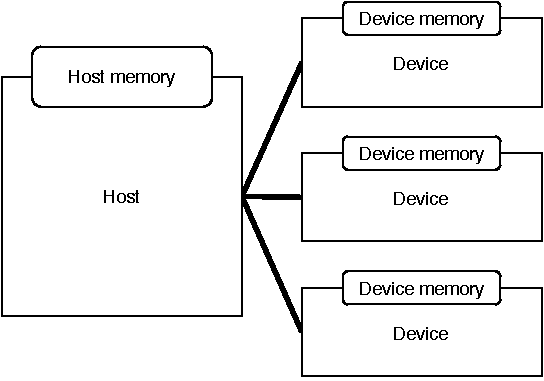
\includegraphics[width=200pt]{\ArtDir/host_device.pdf}}
\caption[The OpenMP host/device model consits of a host processor (typically a CPU) where execution begins, with zero or more attached target devices.
Data and execution can be offloaded from the host to the target device.
The memory spaces are distinct.]
{The OpenMP host/device model consists of a host processor (typically a CPU) where execution begins, with zero or more attached target devices.
Data and execution can be offloaded from the host to the target device.
The memory spaces are distinct.}
\end{figure}

We can query the OpenMP runtime for the number of available target devices in the system using the \texttt{omp\_get\_num\_devices()} API call.

\begin{verbatim}
#include <stdio.h>
#include <omp.h>

int main() {
  printf("There are %d devices\n",
    omp_get_num_devices());
}
\end{verbatim}

\subsection{Target construct offloading execution}
\begin{itemize}
  \item Target directive.
  \item Defines movement of execution to the target device.
  \item Host waits for the region to finish.
  \item Don't want too much detail on the tasking model here because will go into it in Chapter~\ref{chapter:async}. It's not relevant for getting starting this early on.
\end{itemize}

\section{The target memory environment and implicit mapping rules.}
\begin{itemize}
  \item target directive also triggers data movement as well as execution.
  \item first place where data movement is allowed, and will introduce the others at appropriate points.
  \item Different kinds of data we want to move: scalars, (stack) arrays, heap data/pointers, structures.
\end{itemize}

\subsection{Scalar variables}
\begin{itemize}
  \item Mapped as firstprivate.
  \item Example: {\tt int N; double x;}
  \item a scalar struct, as long as it is a complete type
  \item {\bf Not} copied back to the host at end of target region.
\end{itemize}

\subsection{Stack arrays}
\begin{itemize}
  \item Fixed sized stack arrays.
  \item Example: {\tt double arr[1024];}
  \item Complete types. Arrays of structs if complete type.
  \item Copied to device at start of target region, copied back at the end.
  \item Host not allowed to use copy in the meantime (with further details on this in Chapter~\ref{chapter:async}\dots).
  \item Data shared between {\bf all threads} on a device.
\end{itemize}

\subsection{Warning: heap arrays and pointers - reference later chapter}
\begin{itemize}
  \item We don't introduce the map clause yet.
  \item This is done in Chapter~\ref{chapter:memory}.
  \item This section says that we must do something explicit for everything not covered by the implicit rules.
  \item Examples of those would be heap arrays, and data-structures with pointers.
\end{itemize}

\section{Example: Vector add. arrays on stack. No need for map clauses yet.}
\begin{itemize}
  \item Takes vector add example from Chapter~\ref{chapter:overview}.
  \item Arrays are allocated on the stack, so follows implicit mapping rules.
  \item Example will simply transfer execution.
  \item Parallelism comes in Chapter~\ref{chapter:parallelism}.
  \item In OpenCL, have to deal with the host API copying buffers to/from host and device before we can run a meaningful kernel. Thinking in OpenCL might help here.
\end{itemize}

